Salutations!

This article examines four integer sequences which have very interesting properties, beginning with a self-referential sequence described by William Kolakoski in 1965. Its first few terms are: \par
\(1, 2, 2, 1, 1, 2, 1, 2, 2, 1, 2, 2, 1, 1, 2, 1, 1, 2, 2, 1, 2, 1, 1, 2,\)
\\
\(1, 2, 2, 1, 1,\ldots\) \par
Now look at the Kolakoski sequence and construct a new sequence by recording the lengths of the “runs” of consecutive identical integers. For example at the beginning there is a single “1”, so we write down “1”. Then there are two 2s, so we write down another “2”. If you continue this process, you will generate the same sequence! \par
There are many questions that arise when discovering something like this: firstly, does this infinite sequence only contain 1s and 2s? Yes, which can be seen from the fact that new terms of the sequence are generated from the runs of previous parts of the sequence and since no runs of a length greater than two appear in the segment above, we can deduce that no numbers higher than 1 or 2 will ever appear. Secondly, is this sequence unique in this recursive property? \par
No. The sequence works if you omit the first term but, more strongly, we can say that there is an infinite family of these sequences which use different integer sets. For example:\par

\(\{1, 2, 3\}\) generates 1, 2, 2, 3, 3, 1, 1, 1, 2, 2, 2, 3, 1, 2, 3, 3, 1, 1, 2, 2, 3, 3, 3, 1, 2,\ldots

\(\{1, 3\}\) generates 1, 3, 3, 3, 1, 1, 1, 3, 3, 3, 1, 3, 1, 3, 3, 3, 1, 1, 1, 3, 3, 3, 1, 3, 3,\ldots

We can also have infinite sets of integers as “generators”: \par

\(\{2, 3, 5, 7, 11,\ldots\}\) (primes) generates 2, 2, 3, 3, 5, 5, 5, 7, 7, 7, 11, 11, 11, 11, 11, 13, 13, 13, 13, 13, 17, 17, 17, 17, 17, \ldots

This sequence has the property that the \(n^{th}\) term is the number of times \(n\) appears in the sequence: \par
\(\{1, 2, 3, 4, 5,\ldots\}\) generates 1, 2, 2, 3, 3, 4, 4, 4, 5, 5, 5, 6, 6, 6, 6, 7, 7, 7, 7, 8, 8, 8, 8, 9, 9, \ldots

Furthermore, permutations of these sets of integers can create different Kolakoski sequences, which you could check on a notepad. In fact, a great and perhaps unintuitive result is that any sequence of integers, countable in length, in which no two consecutive terms are the same can generate a Kolakoski sequence! \par

So, a relatively simple logical concept has borne all this brilliant fruit and so I present another --- what if a sequence that generates itself through run-lengths could be seen as a 1-periodic point under the function of “run-length encoding”? Describing the Kolakoski sequences we have looked at so far in this manner allows to wonder if there could be 2-periodic sequences or higher…\par

Once again, it is amazingly possible to find examples of this: a sequence whose run-lengths generate a new sequence whose run-lengths generate the first! Here are some examples:\par

A pair which generate each other:\par
\begin{enumerate}
\item \(1, 1, 2, 1, 1, 2, 2, 1, 2, 2, 1, 2, 1, 1, 2, 2, 1, 2, 2, 1, 1,\)\\\( 2, 1, 2, 2, \ldots\)
\item \(2, 1, 2, 2, 1, 2, 1, 1, 2, 2, 1, 2, 2, 1, 1, 2, 1, 1, 2, 1, 2,\)\\\(2, 1, 1, 2, \ldots\)
\end{enumerate}
A miraculous cyclical quintuplet where each sequence in the list generates the one below it:\par
\begin{enumerate}
\item \(1, 1, 2, 2, 3, 3, 4, 4, 4, 5, 5, 5, 1, 1, 1, 2, 2, 2, 2, 3, 3,\)\\\(3, 3, 4, 4, \ldots\)
\item \(2, 2, 2, 3, 3, 3, 4, 4, 4, 5, 5, 5, 1, 1, 1, 1, 2, 2, 2, 2, 3,\)\\\(3, 3, 3, 4, \ldots\)
\item \(3, 3, 3, 3, 4, 4, 4, 4, 5, 5, 5, 5, 1, 1, 1, 1, 2, 2, 2, 2, 3,\)\\\(3, 3, 3, 3, \ldots\)
\item \(4, 4, 4, 4, 4, 5, 1, 1, 2, 2, 3, 3, 3, 4, 4, 4, 5, 5, 5, 5, 1,\)\\\(1, 1, 1, 2, \ldots\)
\item \(5, 1, 2, 2, 3, 3, 4, 4, 4, 5, 5, 5, 1, 1, 1, 1, 2, 2, 2, 2, 3,\)\\\(3, 3, 3, 4, \ldots\)
\end{enumerate}

Try them!\par
To my knowledge, it is not known but conjectured that there exist \(n\)-tuplets of sequences that generate each other as above out of any countable sequence of integers that can be made into a 1-periodic Kolakoski sequence for any natural \(n\).\par

\triast

Self-description can be encoded mathematically in many ways, often leading to complex or chaotic behaviour and the Kolakoski sequence (the original version) is a good example: it is conjectured that the sequence is aperiodic i.e. it never repeats. Gijswijt’s sequence, named after the mathematician Dion Gijswijt, is another such encoding…\par
To explain the process of determining the \((n+1)^{th}\) term of the sequence, one needs to understand strings and basic string notation. A string is simply a series of characters (not limited to numbers) written next to each as if the letters of a word. The process of taking an ordered collection of such characters and writing them together in this manner is referred to as concatenation (this word generally means the combination of any strings \(X\) and \(Y\) into \(XY\)). If \(Y\) is a string, then we denote \(Y\) repeated \(k\) times as \(Y^k\).\par
Thus, given the first \(n\) terms of Gijswijt’s sequence, consider concatenating them into a string which can be denoted as \(XY^k\), where \(Y\) is the largest “block” within the string that is repeated at the end and \(X\) is the rest of the string. The \((n+1)^{th}\) term is \(k\). To illustrate, let us go through the creation of the first few terms together.\par

\begin{figure}
\caption{Graph of the first few terms of Gijswijt's Sequence}
\centering
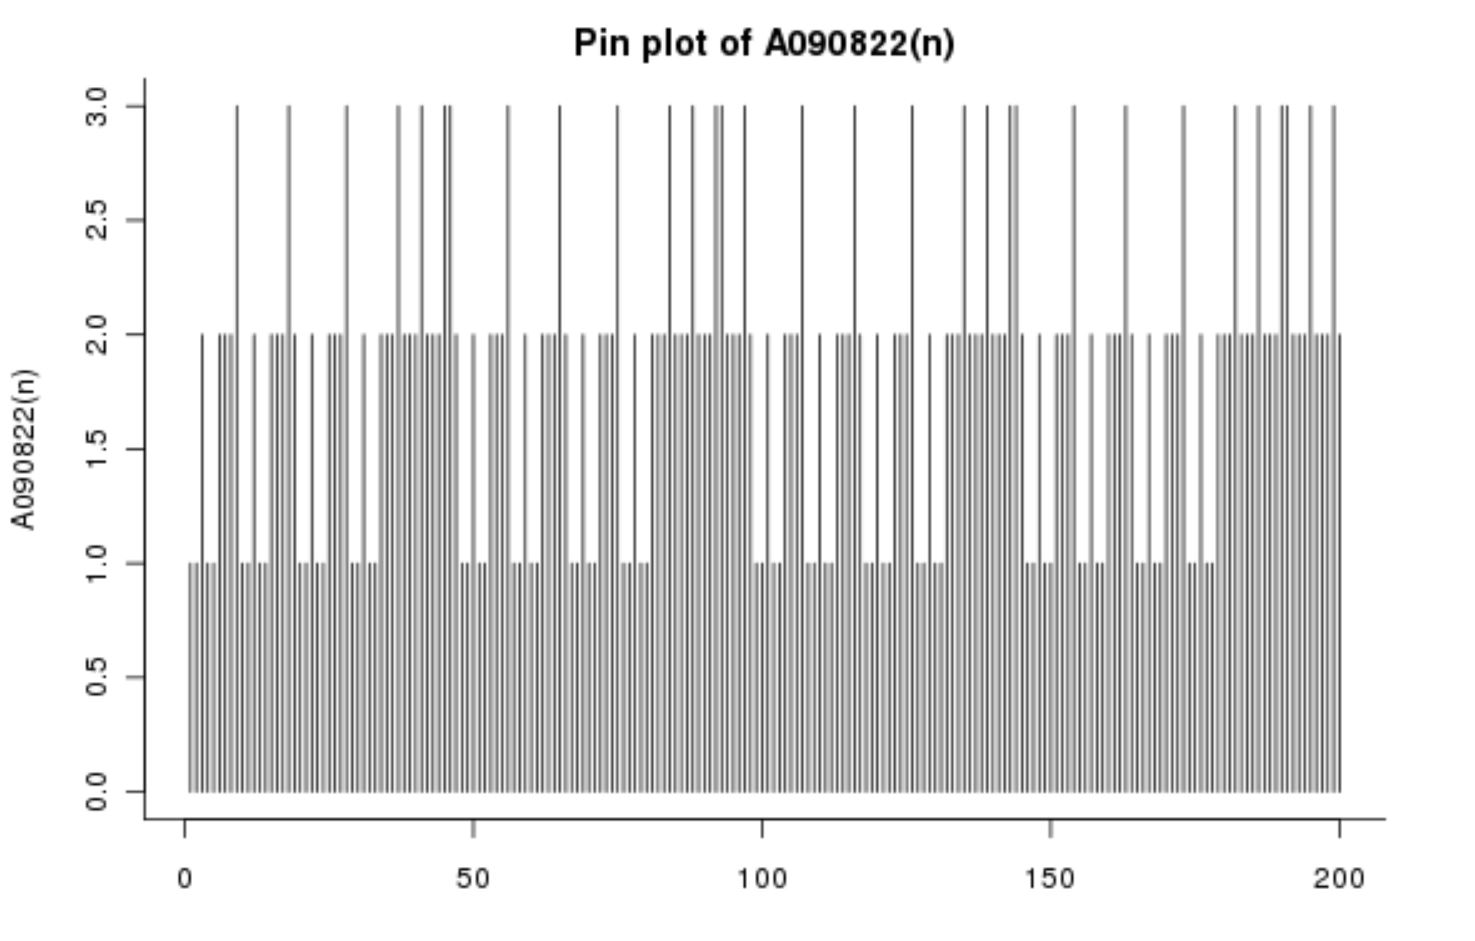
\includegraphics{Gijswijt.JPG}
\end{figure}

Originally, we have nothing and since that nothing is “repeated once” (it is the \(Y\) for this string), we write 1 as the first term. Since 1 is repeated only once so far, we write another 1. Now, as there are two 1s in succession, we write down 2. See if you can understand the rest here:\par

\[1, 1, 2, 1, 1, 2, 2, 2, 3, 1, 1, 2, 1, 1, 2, 2, 2, 3, 2, 1, 1, 2, 1, 1, 2, \ldots\]

Reasoning about it is not simple at first --- for example, you see how 1,1,2 appears twice and then is followed by a 2 to represent the repetition of that entire block, then by another 2 to represent the two 2s next to each other… In fact, it is this nontrivial “block and glue” structure that is key to its understanding:\par
Let’s refer to Gijswijt’s Sequence as \(G_1\) and then observe that the entire sequence is made up of “blocks” that are doubled and then are ended with some sort of “glue” sequence, for example the first block \(B_1\) is 1 and the first glue \(E_1\) is 2 since we begin with 1,1,2. The next block, \(B_2\), is 1,1,2 (or \(B_1B_1E_1\)) and the next glue sequence is 2,2,3. We can generalise this to larger blocks and glue sequences: \(B_{n+1} = B_nB_nS_n\) where \(S_n\) is simply defined to be the sequence of numbers starting at the end of \(B_nB_n\) and ending at the first 1 reached.\par
What’s interesting about this analysis is that one can combine all the glue sequences into a new infinite sequence, \(G_2\), which follows the same \((n+1)^{th}\) term rule as \(G_1\) except instead of writing the \(k\) from \(XY^k\), we write \(max\{k, 2\}\). Here are the first 25 terms:\par

\(2, 2, 2, 3, 2, 2, 2, 3, 2, 2, 2, 3, 3, 2, 2, 2, 3, 2, 2, 2, 3, 2, 2, 2,\)\\\( 3, \ldots\)

One can perform similar structural analysis on \(G_2\) as above and further construct a \(G_3\) and more generally, \(G_n\). We can observe that every \(G_n\) starts with \(n\) and so, perhaps surprisingly, prove that Gijswijt’s Sequence is unbounded (that is, there is no finite positive integer that does not appear at some point in the sequence). However, it should be noted that the sequence grows exceptionally slowly, with \(n\) believed to generally appear at roughly the\par

\[2^{3^{4^{5^{\ldots^{n}}}}}\textrm{th}\]

term and thus, despite its unboundedness, is conjectured to have a finite average!\par

\triast

Our next phantasmagorical sequence was first investigated by the lesser known (and yet important) combinatoricist and number theorist James Joseph Sylvester. It begins\par

\[2, 3, 7, 43, 1807, 3263443,\]
\[10650056950807,\]
\[113423713055421844361000443, \ldots\]

One constructs the \((n+1)^{th}\) term by taking the product of the first \(n\) terms and adding one --- you can see this above. Equivalently, one can define it, where \(s_n\) is the \(n^{th}\) term of the sequence, as\par

\[s_n = s_{n-1}*(s_{n-1}-1)+1 \textrm{ with } s_0 = 2\]

\begin{figure}[h!]
\caption{Graph of the first few terms of Sylvester's Sequence}
\centering
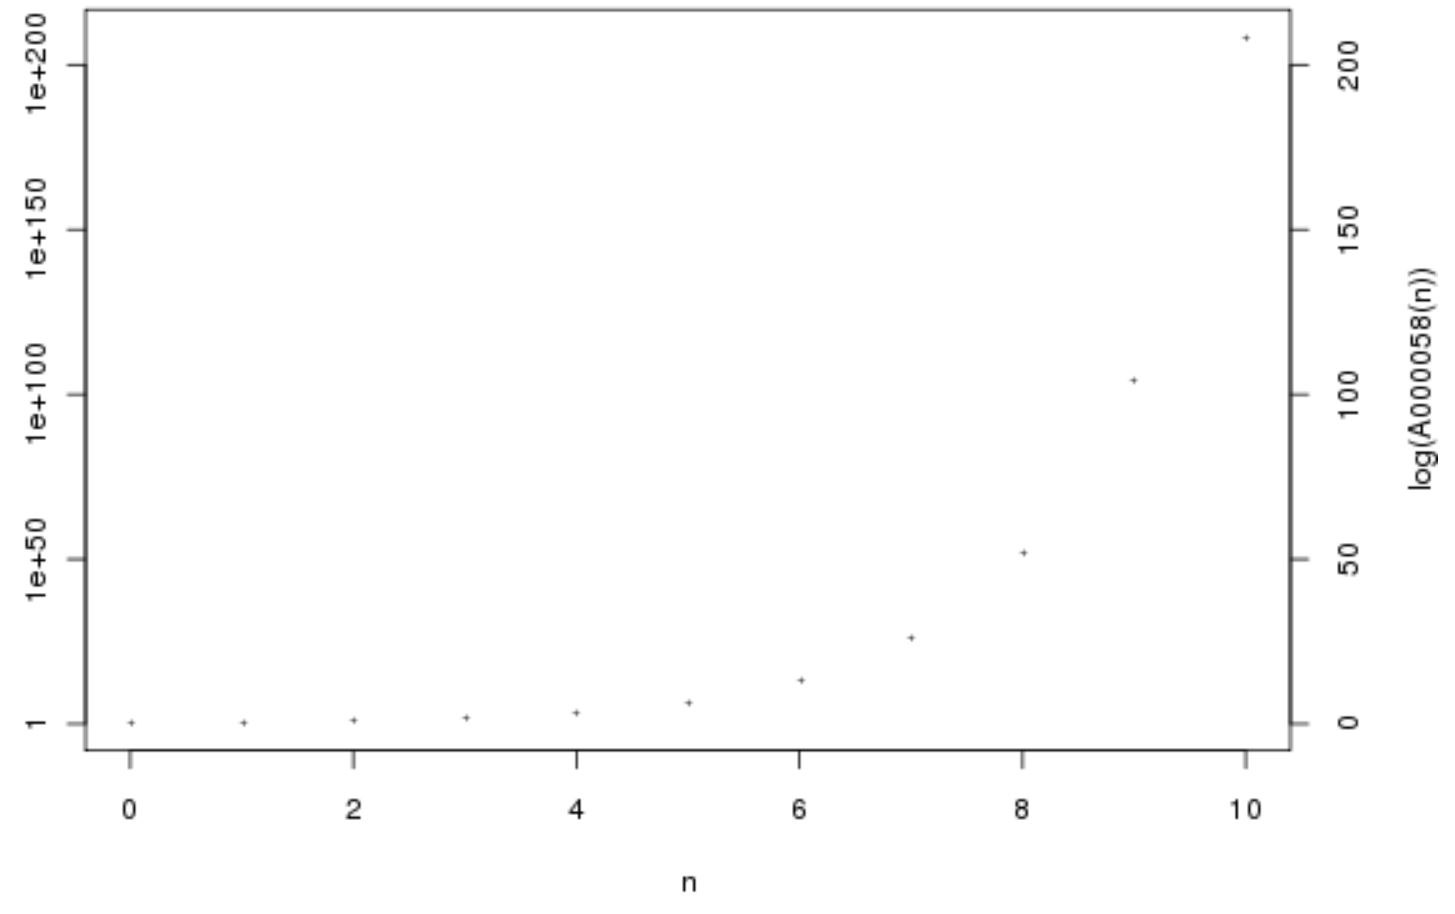
\includegraphics{Sylvester.JPG}
\end{figure}

The fact that these two definitions are equivalent can be seen given some quick thought. Let us consider the sum of the reciprocals of the terms in Sylvester’s sequence. We can first see definitionally that\par

\[\frac{1}{s_i-1}-\frac{1}{s_{i+1}-1} = \frac{1}{s_i-1}-\frac{1}{s_i(s_i-1)} = \frac{(s_i-1)}{s_i(s_i-1)}\]
\[ = \frac{1}{s_i}\]

Thus, we can use the concept of telescoping (described by Euler as the “method of differences”) to see that\par

\[\sum^{j-1}_{i=0} \frac{1}{s_i} = \sum^{j-1}_{i=0} (\frac{1}{s_i-1} -\frac{1}{s_{i+1}-1})\]
\[ = (\frac{1}{s_0-1} -\frac{1}{s_{j}-1}) = 1 - \frac{1}{s_{j}-1} = \frac{s_j-2}{s_{j}-1} \]

We can deduce from the last two equivalences an impressive result: since Sylvester’s sequence obviously tends to infinity, the sum of the reciprocals of its terms tends to 1! Furthermore, the last equivalence in particular tells us that if we were to sum up to the \(j^{th}\) term in the sequence and subtract one from the last denominator, we would also get one, since\par
\[ \frac{s_j-2}{(s_{j}-1)-1} = 1\]

Thus, we can see that:\par

\[ 1 = \frac{1}{2}+\frac{1}{3}+\frac{1}{6}\]
\[ 1 = \frac{1}{2}+\frac{1}{3}+\frac{1}{7}+\frac{1}{42}\]
\[ 1 = \frac{1}{2}+\frac{1}{3}+\frac{1}{7}+\frac{1}{43}+\frac{1}{1806}\]
…
This allows us to have a different interpretation of Sylvester’s sequence: a “greedy algorithm” which at each stage, chooses the smallest \(n\) such that \(\frac{1}{n}\) plus the partial sum of the reciprocals of all the terms so far is less than one. This allows us to see that it is the fastest converging-to-one series of unit fractions and also allows us to consider other Sylvester-esque sequences. For example, what about the greedy algorithm series formed from \(s_0 = \frac{1}{4}\) and the limit being 2? I was able to compute these 6 terms on my computer:\par

\[2, 2, 5, 21, 421, 176821, \ldots\]

You can see that the recurrence relation that held with Sylvester’s sequence also holds here! Furthermore, if one tries to derive similar convergent sequences to rational numbers using the greedy algorithm, one will often observe a “Sylvestrine” relation. This is all due to a result obtained by modern mathematician, Badea, which states that if one has a sequence of integers \(a_n\) such that \(a_n \geq a_{n-1}^2-a_{n-1}+1\) and the sum of its reciprocals converges to some rational number, then after some finitely reachable point in the sequence the terms will follow the recurrence relation that defines Sylvester’s sequence --- there is something fundamental about it to doubly exponential series…\par
Investigations into its closed-form (non-recursive) representation have led to the surprising discovery that there exists what we shall name the Sylvester Constant \(E\) such that\par

\[s_n = \left \lceil{E^{2^{n+1}}+\frac{1}{2}}\right \rceil\]

with \(E = 1.26408\ldots\).

\triast

We finish off with a fun sequence investigated by the British mathematical jack-of-all-trades, John Horton Conway. He recalls that a student once excitedly thrust a sheet of paper under his nose with these 5 terms on it:\par

\[1, 11, 21, 1211, 111221, \ldots\]

and he was asked to guess the next number in the sequence. He was not able to do this, however, and after some guesses and deliberation the student revealed to him the rule for constructing the rest of the sequence. What he called the Look and Say numbers were made by reading through the previous term, counting those groups of consecutive numbers which are the same. For example, starting with “1”, we would say that there is “One 1” and thus the next term is “11”. For something more complicated like “1211”, we say there is one “1”, followed by one “2” and then a final grouping of two “1”s: thus “11 12 21” concatenated, or “111221”.\par

\begin{figure}[h!]
\caption{Graph of the first few terms of Look and Say}
\centering
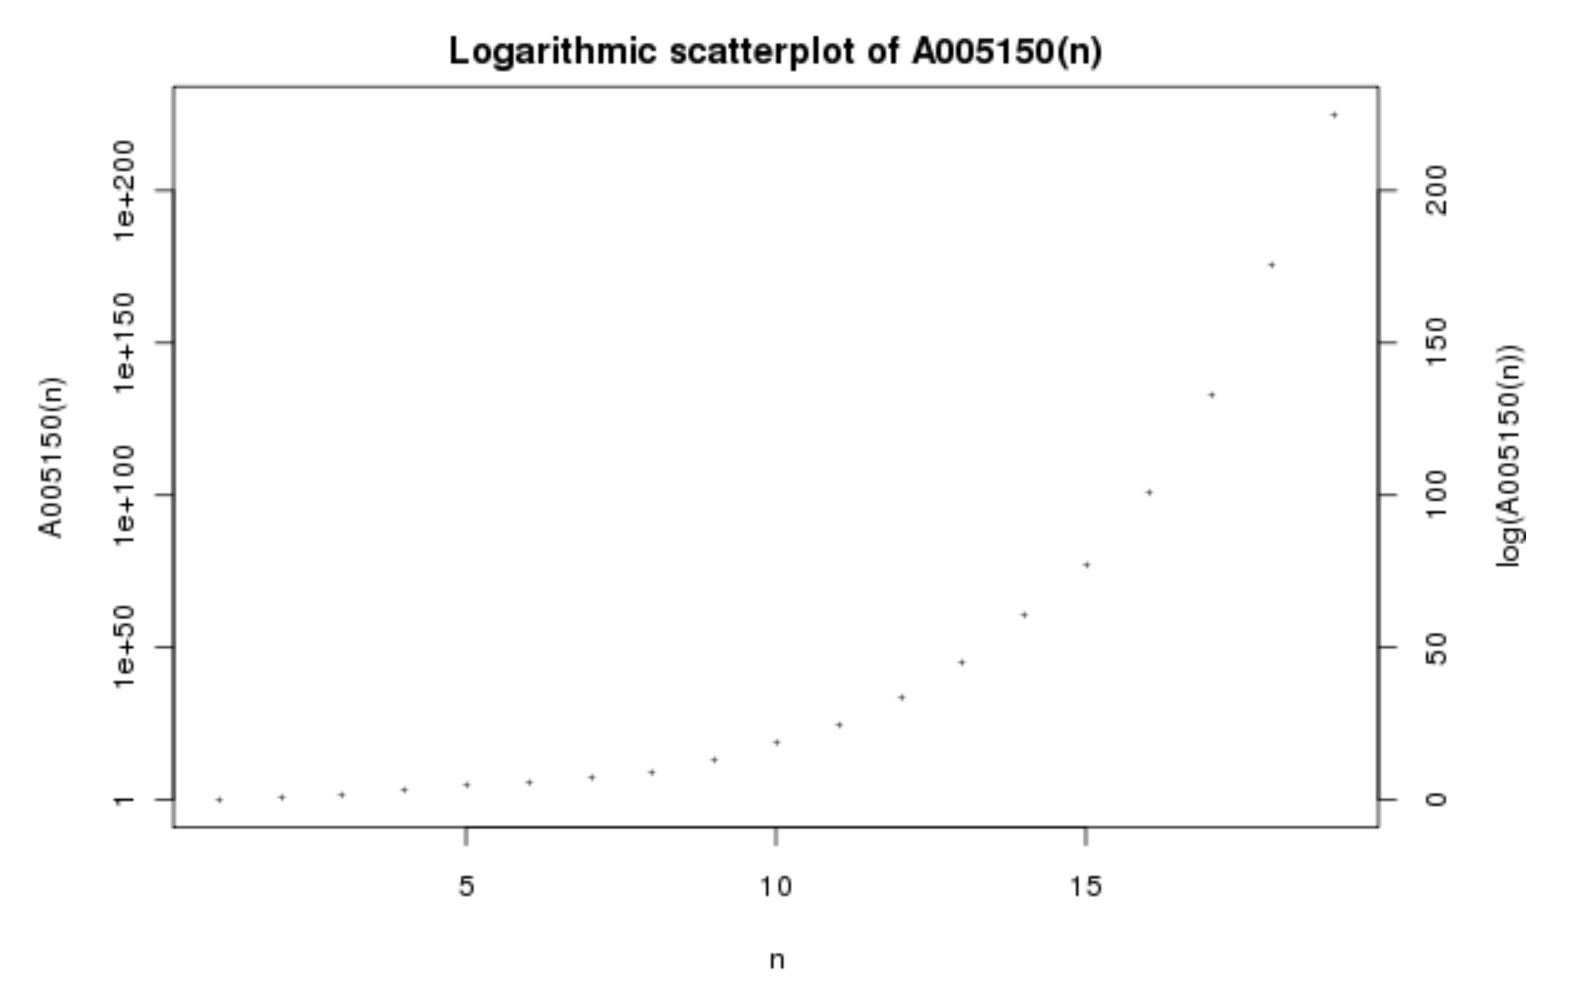
\includegraphics{LookAndSay.JPG}
\end{figure}

Conway took some time later to investigate the properties of this seemingly arbitrary recurrence relation and the many sequences that one could generate from different starting integers. What was immediately apparent was that any sequence apart from the anomalous “22, 22, 22, \ldots” would be divergent (tend to infinity) and that for any digit \(n \neq 1\), the sequence would be

\[n, 1n, 111n, 311n, 13211n, \ldots\]

with \(n\) forever staying at the end. He then came upon and proved two remarkable results, which he published in his brilliantly titled paper The Weird and Wonderful Chemistry of Audioactive Decay. The first was the celebrated Cosmological Theorem, which states that after some finite point, any look-and-say sequence splits into a discrete grouping of strings, whose dynamics are independent beyond this point. It turns out that there are only 92 of such strings that only involve 1s, 2s \& 3s, so he called them “elements” (after all, how many naturally occur?) and referred to this process of sequence bifurcation as “audioactive decay”. The elements involving digits other than just 1, 2 or 3 were called “transuranic” since their abundance in a given \(n\)-length string tends to zero as \(n\) tends to infinity (they don’t change beyond just appearing as “\(1n\)”). Transuranic elements in real life have an extremely short half-life, so this further extends the wit of the nomenclature!\par
The table of elements is too large to be shown here (having 92 rows!) but I urge you to look it up! After all, the mechanics of any look-and-say sequence is after a point (maximally, the 8th term) completely determined by these elements and furthermore, by examining the lengths of all the elements, we can precisely predict the change in the length of the term.\par
Suppose we construct a 92 by 92 matrix in which entry \((x, y)\) is equivalent to the product of the number of times the \(x^{th}\) “element” appears in the decay-successor to the \(y^{th}\) “element” and the ratio of the lengths of the \(x^{th}\) and \(y^{th}\) “element”s. Then, consider representing the length of a given term \(T\) in a look-and-say sequence as a vector whose \(n^th\) item is the length of the \(n^{th}\) “element” multiplied by the number of times it appears in \(T\).\par
By multiplying the “length vector” by the matrix, we get a new vector which encodes the length of what would be the next term in the look-and-say sequence. From this, Conway was able to calculate an invariant of the matrix known as its characteristic polynomial. This allowed him to deduce a new theorem…\par
If one looks at look-and-say sequence terms’ lengths, you can see that they increase exponentially. Below is a logarithmically-scaled graph of the length of terms in the traditional look-and-say sequence starting with 1.\par

\begin{figure}
\caption{Logarithmic graph of a length of Look and Say terms}
\centering
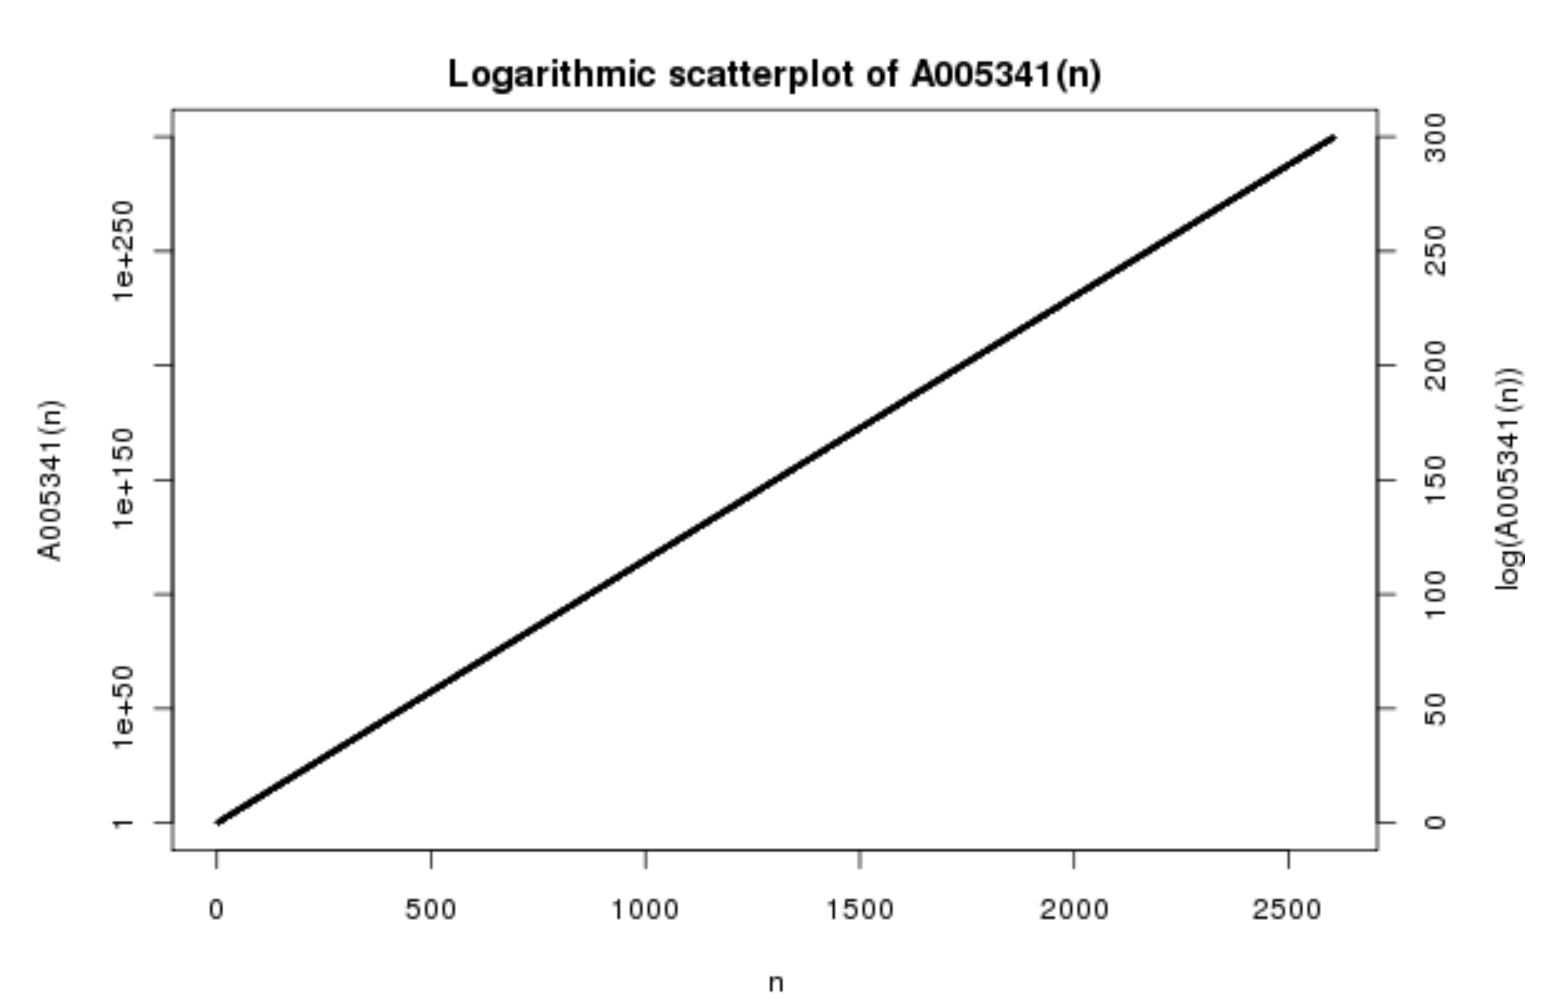
\includegraphics{LookAndSayLength.JPG}
\end{figure}

The amazingly straight line means that the length of terms scales by an almost constant value, due to the logarithmic scale on the y-axis, across the sequence. This is intriguing --- basic investigation reveals that it is roughly 30\% increase each term. What Conway deduced from the characteristic polynomial of the aforementioned matrix was the precise value of this scale factor, 1.303577269\ldots, which is its only positive real root!\par
This astounding result suggests that the look-and-say generation rule, far from being arbitrary, is apparently very ordered. It led to Conway proclaiming that this investigation was the “most complicated solution to the simplest problem” that he had ever seen.\par
To conclude, I wanted to mention an amazing resource which slips beneath the radars of full-time and recreational mathematicians alike at our age: the Online Encyclopaedia of Integer Sequences. Nearly all the terms and sequences mentioned in this article I only found out due to the OEIS; most of the graphs in this article were taken from the OEIS’s graph tool for sequences. The OEIS was set up in the 2000s as the result of a 40-year project that had been run by Neil Sloane, a number theorist particularly interested in integer sequences --- indeed, the title of this article is taken from a talk of the same name given to a computer science group at Princeton University this year.\par
The OEIS has reference codes for all its sequences in the form “AXXXXXX”, which allow you to easily what you are looking for on their website. For further reading or your own investigations, here are the OEIS codes for the sequences mentioned in this article:

\begin{itemize}
\item{\textit{Kolakoski Sequence}, A000002}
\item{\textit{Gijswijt’s Sequence}, A090822}
\item{\textit{Sylvester’s Sequence}, A000058}
\item{\textit{Look-and-say Sequence} (starting with 1), A005150}
\end{itemize}

Finally, we couldn’t finish an ARM article without challenges. As per usual, this article was written by Isky Mathews but feel free to email your answers to the other author Benedict Randall Shaw.

Challenge IV:
\begin{enumerate}
\item{Investigate other “Sylvestrine” greedy sequences as mentioned --- can you create an infinite number of different representations of the number they converge to as finite sums of unit fractions like above?}
\item{Create a formula for the \(n^{th}\) term of the traditional Kolakoski Sequence (it can be recursive!). Using this, record the relative frequency of 1s and 2s in the sequence up to some large \(n\) via a computer program implementation. Make a conjecture of what fraction of the sequence’s terms are 1s based on this.}
\end{enumerate}
